% Report of results from Ramsay simulation experiment
% David Lawrence Miller
% d.l.miller@bath.ac.uk

% Started : 29 October 2008

\documentclass[a4paper,10pt]{amsart}

% Load some packages
\usepackage{times, amsmath, amssymb, amsfonts, url, natbib, bm, rotating,multirow,graphicx}

% top matter
\title{Smoothing over the Ramsay horseshoe using the Schwarz-Christoffel transform}
\author{David Lawrence Miller}
\email{d.l.miller@bath.ac.uk}
\address{Mathematical Sciences, University of Bath, Bath, United Kingdom}

% Shortcuts
% Probability
\newcommand{\prob}[1]{\mathbb{P}\left[ #1 \right]}
% Hovitz-Thompson
\newcommand{\HT}{\hat{\tau}_{HT}}
% Schwarz-Christoffel
\newcommand{\sch}{Schwarz-Christoffel }
% fprime
\newcommand{\fprime}{f^\prime(z)}
% figure reference command
\newcommand{\fig}[1]{\emph{fig.} (\ref{#1})}
% figure reference command (start of sentance
\newcommand{\Fig}[1]{\emph{Fig.} (\ref{#1})}
% equation reference command
\newcommand{\eqn}[1]{\emph{eqn.} (\ref{#1})}
% phi inverse
\newcommand{\phiinv}{\phi^{-1}}
% use other phi
\newcommand{\ophi}{\phi}
\renewcommand{\phi}{\varphi}




\begin{document}

% The abstract
\begin{abstract}
Here I investigate an alternative method for smoothing over 2-D regions based on the Schwarz-Christoffel transform from complex analysis. The transform takes the region and ``morphs'' it to a rectangle or disk in a prescribed way. We may then smooth over the transformed area using penalized regression splines. Finally, the smooth is transformed back to the original domain in order to perform analysis. I explore the utility of this transform for the horseshoe shape proposed by \cite{ramsay}.
\end{abstract}


% New theorem for theorems
\newtheorem{thm}{Theorem}[section]

%New theorem for definitions
\newtheorem{defn}{Definition}[section]

\maketitle



\section{Ramsey's horseshoe}

\cite{ramsay} proposes a function which can be used to benchmark new approaches to 2-dimensional smoothing. The function takes the form of a horseshoe which is flat across the domain but ranges from $-4$ to $4$ along the domain's major axis. The so-called ``Ramsay horseshoe'' is shown in \fig{ramsayshorseshoe}.

The test function highlights a common problem in spatial smoothing: that of ``leakage''. When the problem is specified in Euclidean distance, the model thinks that the distance between the $-4$ and $4$ points of the horseshoe is the distance over the gap in between them, rather than the distance along the major axis of the shape. This causes the high density from one side to contaminate the other (or the low to contaminate the high.) It is easy to see that this causes the smooth to be calculated incorrectly.

\Fig{tpleakage} shows what happens when a thin plate spline is fitted to the horseshoe with no information about the structure of the domain. Comparing the contour lines to those in the actual horseshoe, one can easily see that there is leakage.



\begin{figure}
\centering
% trim order l b r t
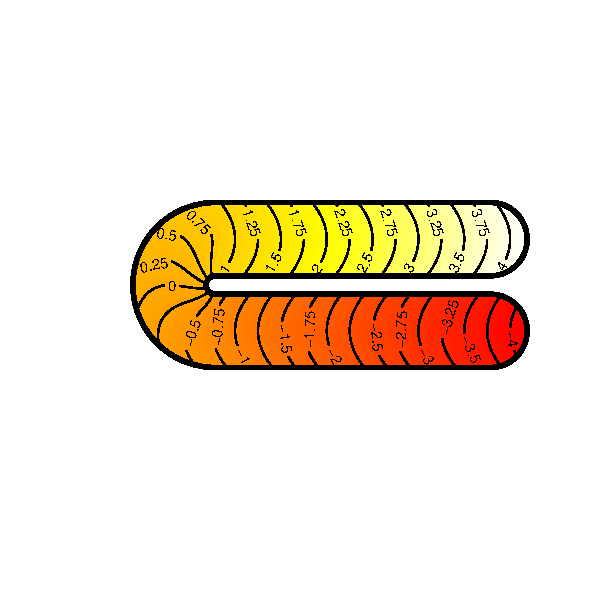
\includegraphics[trim=0.5in 1in 0in 1in]{figs/ramsayhorseshoe.pdf} \\
\caption{Heatmap of the Ramsay horseshoe.}
\label{ramsayshorseshoe}
% generated by /phd-smoothing/sc-writeup/figs/horseshoeplot.R
\end{figure}

\begin{figure}
\centering
% trim order l b r t
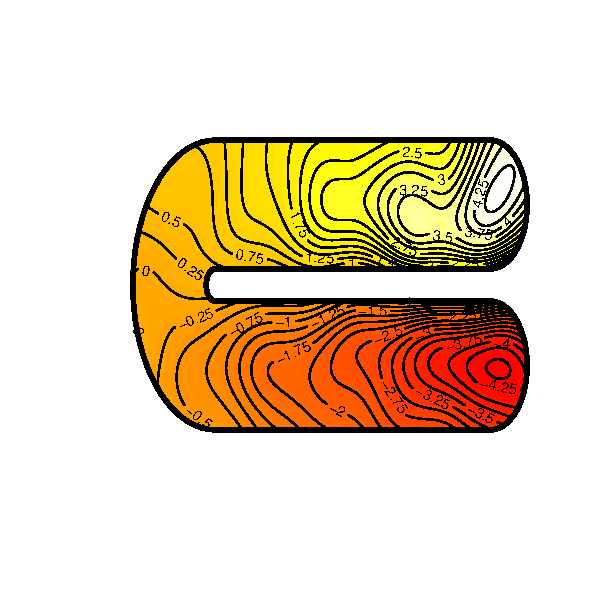
\includegraphics[trim=0.5in 1in 0in 1in]{figs/leakageexample.pdf} \\
\caption{An example of leakage when using a thin plate spline.}
\label{tpleakage}
% generate /phd-smoothing/sc-writeup/figs/tpramsayfit.R
\end{figure}

Clearly we would like to use an approach that respects the shape of the region, taking into account the structure of the domain and does not show any evidence of leakage. In order to deal with the problems of a complex region, four different approaches have been proposed:

\begin{enumerate}
\item \cite{ramsay} proposes finite area $L$-splines (FELSPLINEs.) The $L$-spline has a differential operator in its penalty, which cannot be analytically solved in two dimensions. However, to combat this, the author triangulates the domain and then constructs a set of bivariate quadratic polynomial basis functions over each triangle, specifying that there be continuity over the edges of the triangles. The union of these functions is then a solution to the PDE in the penalty and therefore the solution to the usual smoothing objective function\footnote{\emph{ie.} $\sum_{i=1}^n (z_i-f(x_i,y_i;\theta))^2 + \lambda \int_\Omega Pf(x,y;\theta)d\Omega$, where $P$  is some penalty operator}.

Although it performs better than previous models on the horseshoe, FELSPLINE does not do very well in practice. This is since its boundary conditions specify that the gradient is normal to the edge of the area. This is not always physically realistic.

\item \cite{wangranalli} adopt a ``within-area distance'' formulation for thin plate splines. In this case they take the geodesic distance between two points, that being the shortest path within the domain. This gives a definition of how near objects are in the domain.

Since the geodesic distance is only known if the intrinsic structure of the domain is known (which is rare in ecological examples), the authors use a different method to calculate the shortest path. For this they create a graph, with datum at each node and the distance between each pair of nodes as the weights on the edges. Floyd's algorithm\footnote{Which is cubic in the number of vertices.} is then used to find the $k$ nearest neighbors of each node.


\item \cite{soap} consider constructing a soap film over the domain. The film is then weighed down by the data, the objective is then to minimize the surface tension in the film.

\item An alternative approach is to ``morph'' the area in question to be one which is more suitable for smoothing. For example, with Ramsay's horseshoe, it seems intuitive to simply bend the horseshoe into a long strip and then smooth on that domain. This is what we propose here. 

This approach raises some questions. First, what is the natural domain to transform to? Second, what is the nullspace of this new domain? Clearly for some shapes the answer to both of these questions is obvious, but this is not always the case. We address these problems below.


\end{enumerate}




\section{Method}

Here we formulate a conformal mapping from the domain of the problem (we call this the $W$ domain) to a domain on which it is easier to smooth (which we denote $W^*$.) We elaborate on what was alluded to in \cite{eilerstalk}: using the \sch mapping to transform our domain to another in order to perform smoothing. Our hope is that by using our approach we can avoid the problems detailed above.

\subsection{\sch}

The \sch transform provides a way to map an arbitrary polygon in the complex plane to one of a set of objects (also in the complex plane.) The two most commonly mapped to objects are the unit disk and the rectangle. The procedure consists of adding vertices to the object you wish to map to and then deforming it iteratively until it is identical to the polygon. More formally we wish to find $\phi: W \mapsto W^*$.

For example: we wish to transform between a regular nonagon and a rectagle. We add five sides to the rectangle and then go about deforming it to the shape of the nonagon (by changing the angles at the vertices and then rescaling and rotating it as necessary.) 

\Fig{hsgridmapping} shows how a grid of points in the horseshoe are re-mapped. We see that the density of the grid once it has been mapped has become non-uniform. This presents the aforementioned problem of calculating the nullspace of the penalty, \emph{ie.} what is the line that is unpenalised in our model?

Note that although we have gone from one domain with a peninsula to another, also featuring a peninsula. However, a considerable improvement has been made on the concavity of the region. 

\begin{figure}
\centering
% trim order l b r t
\begin{tabular}{cc}
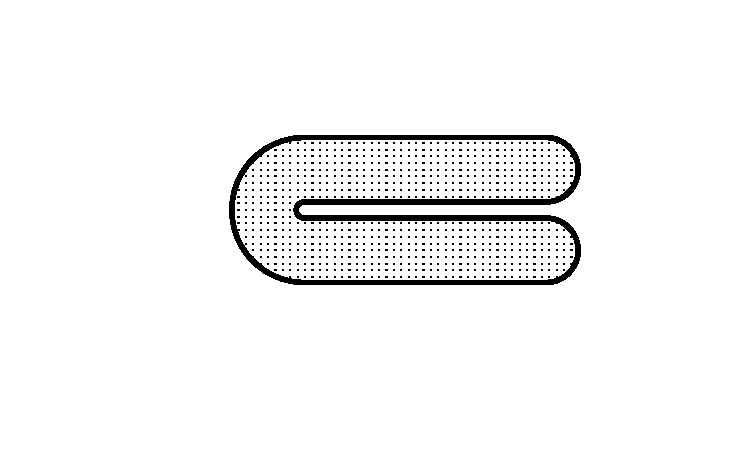
\includegraphics[height=0.75in, trim=1in 1in 0in 0.75in]{figs/hsgridmapping-1} & 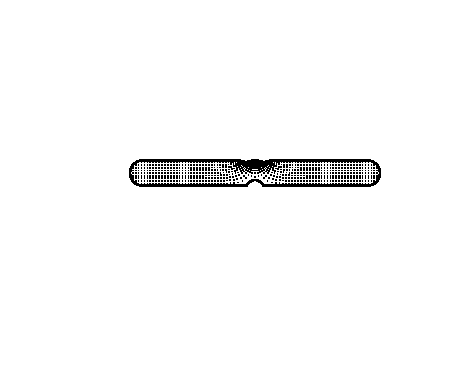
\includegraphics[height=0.75in, trim=1in 1in 0in 0.75in]{figs/hsgridmapping-2} \\
\end{tabular}
\caption{The mapping of a regular grid from the horseshoe under the \sch transform. The diagram was created by generating the grid over the bounding box in \fig{hswithboundingbox}, dropping those points not in the horseshoe and then mapping the points.}
\label{hsgridmapping}
% generated by /phd-smoothing/sc-writeup/figs/hsgridmapping.R
\end{figure}

Full technical details of the \sch mapping are given in \cite{miller08}.


\subsection{P-splines}
P-splines (\cite{eilersmarx96}) were used as the basis functions for the smooth since they present an easy framework for adding arbitrary penalties\footnote{Which may become useful if distortions to the polygon become problematic.}. P-splines are essentially a B-spline basis with a penalty which provides a discrete approximation to the (standard) integrated $k^\text{th}$ derivative of the function. The penalty is given by:

\begin{equation*}
\lambda \sum_{j=k+1}^n (\Delta^k a_j)^2,
\end{equation*}

where $n$ is the number of B-splines, $k$ the derivative we wish to approximate, $a_j$ the coefficient of the $j^\text{th}$ basis function and $\Delta a_j = a_j-a_{j-1}$ and hence $\Delta^2 a_j = a_j-2a_{j-1}+a_{j-2}$. $\lambda$ is the usual smoothing parameter. 

\subsection{Thin plate regression splines}
Thin plate regression splines (\cite{simonbook}, \emph{pp. 154-159}) provide a framework for smoothing in which knots do not to have to be selected and an implicit definition of smoothness is built into the model.

As thin plate splines are isotropic smoothers it is not expected that the thin plate splines will do very well on the Ramsay test function since the test function is only varies along one axis. Thin plate splines are used here mainly as a comparison to the P-splines to assess whether the the P-spline's performance is due to the natural advantage of tensor product over isomorphic smoothers in such situations.

\subsection{Procedure}

Our procedure consists of the following steps:

\begin{enumerate}
\item Determine the domain over which we would like to smooth, $W$. This could be the region or a bounding box around it.

\item Compute the \sch transform of $W$ to get $W^*$. To obtain the function, $\phi$.

\item Map the co-ordinates of the datapoints in $W$ to $W^*$.

\item Fit the GAM to the data in $W^*$.
\end{enumerate}

At this point it depends on the application as to whether a transform is needed to go back to $W$. If we are only interested in, say, the density of a biological population, then this can be estimated in the transformed domain. On the other hand, it may be the objective to obtain other information; for example a graphical representation of the density, in which case the back-transform is required.

\subsection{Software}

There are several pieces of software available to perform the \sch mapping. The Fortran library \texttt{SCPACK} is the oldest available package\footnote{\texttt{SCPACK} can be downloaded from Netlib.} and was used initially. However, it only offers the mapping to the unit disk and does not include the CRDT method for performing the mapping (see \cite{miller08}, section (4.2).) For this reason the SC toolbox (\cite{driscoll}, \emph{pp. 115-119}) for Matlab is used to perform the mapping. 

The \textsf{R} library \texttt{mgcv} provides subroutines for fitting generalized additive models and, in particular, P-splines.

Although packages are available to enable \textsf{R} to talk to Matlab and vice-verse, for the purposes of this exploratory work CSV files were written by each program and read in by the other.

\section{Mapping the Ramsay horseshoe}

In order to map the horseshoe, we first draw a rough bounding box around the shape. Rather than trying to approximate the curved edges with many straight lines, we use the bounding box as the $W$ domain remapped via the \texttt{evalinv()} function from the SC Toolbox. This is shown in \fig{hswithboundingbox}.

\begin{figure}
\centering
% trim order l b r t
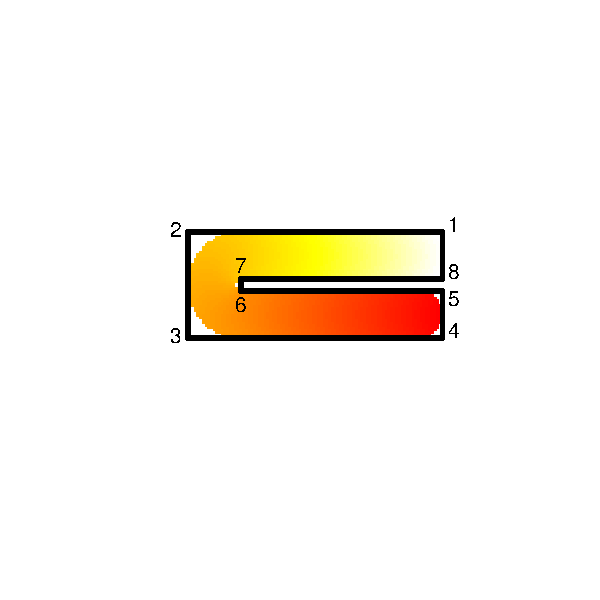
\includegraphics[trim=0.5in 1in 0in 1in]{figs/hswithboundingbox.pdf} \\
\caption{The horseshoe with it's bounding box. Vertices 1, 4, 5 and 8 are mapped to the corners of the rectangle.}
\label{hswithboundingbox}
% generated by /phd-smoothing/sc-writeup/figs/hswithboundingbox.R
\end{figure}

We then transform our bounding box into the rectangle. This is done using the \texttt{rectmap()}\footnote{or \texttt{crrectmap}, its CRDT equivalent (see \cite{miller08}.)} function from the SC Toolbox in Matlab. This function solves the \sch parameter problem as detailed in \cite{miller08}.

A sample of 1000 points from the horseshoe was then taken and noise added to the data. First the $x,y$ coordinates of the sampled points were expressed as complex numbers of the form $w=x+iy$. Then ampping was then performed. This created a new set of coordinates $w^*=x^*+iy^*$. Smoothing was then performed over the responses in the $W^*$ domain using the \texttt{gam()} function in \texttt{mgcv}. 

Comparing the left hand figure in \fig{compsmooth} with \fig{ramsayshorseshoe} we see that transforming the domain gives quite a good approximation to the true figure.

\Fig{compsmooth} shows a comparison between the predicted smooths given by the \sch transformed smooth (using a P-spline basis) and the smooth provided by the soap film smoother. 

%The boxplots in \fig{scvssoapboxplot} show the per point mean squared error over a 100 by 50 call prediction grid.

\begin{figure}
\centering
% trim order l b r t
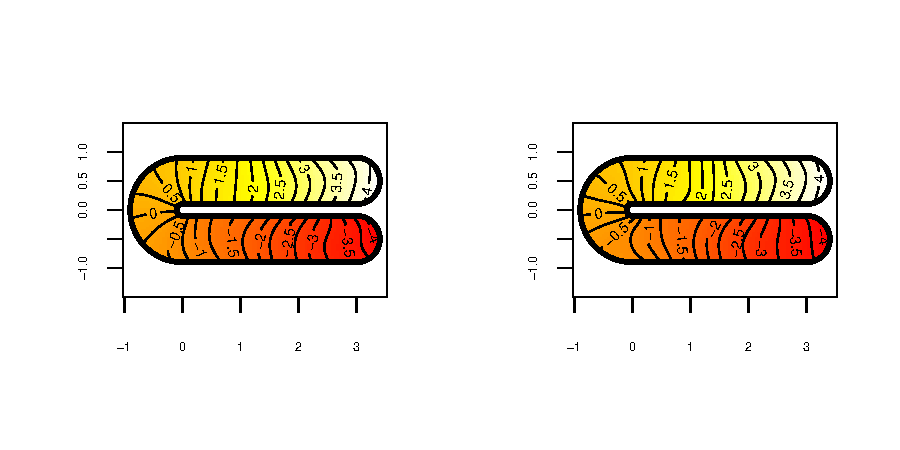
\includegraphics[trim=0.5in 0.5in 0in 0in]{figs/compsmooth.pdf} \\
\caption{Comparison of smooths given using P-splines on the transformed domain (left), thin plate splines on the transformed domain (centre) and soap film smoother (right.)}
\label{compsmooth}
% generated by /phd-smoothing/sc-writeup/figs/pspline.soap.comp.hs.R
\end{figure}

%\begin{figure}
%\centering
%% trim order l b r t
%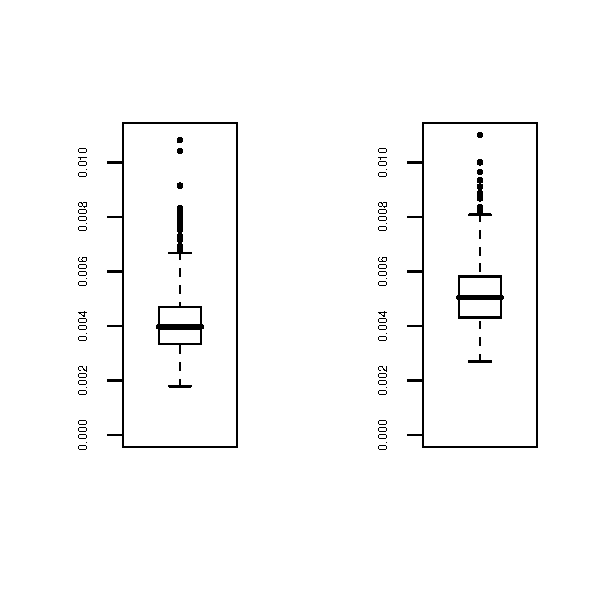
\includegraphics[trim=0.5in 0in 0in 0in]{figs/scvssoapboxplot.pdf} \\
%\caption{Boxplots of mean squared error over the prediction grid. The left plot is for the transformation with P-splines (MSE 0.0041), centre plot is for the transform with thin plate splines (MSE 0.0041), and the right is the soap film smoother (MSE 0.00517.)} 
%\label{scvssoapboxplot}
% generated by /phd-smoothing/sc-writeup/figs/pspline.soap.comp.hs.R
%\end{figure}

Looking at the predicted values for the model in the $W^*$ domain we get an indication as to why the fit is so good. \Fig{hsvisgam} shows the fitted surface and there we can see that there is a strong linear trend along the major axis of the horseshoe, making this a rather trivial smoothing problem. So, it looks like we are addressing the problem in a more natural domain. In the next section we investigate this further.

\begin{figure}
\centering
% trim order l b r t
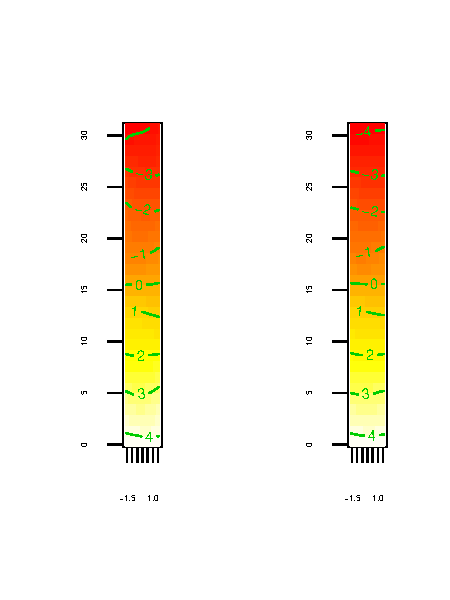
\includegraphics[trim=0in 0.5in 0in 0in]{figs/hsvisgam.pdf} \\
\caption{Heatmap produced by \texttt{vis.gam} for the smooth over the horseshoe in the transformed domain using P-splines (left) and thin plate splines (left).}
\label{hsvisgam}
% generated by /phd-smoothing/sc-writeup/figs/hsvisgam.R
\end{figure}

\subsection{Problems}

As mentioned above, when the domain has been morphed it is not clear what the definition of smoothness is, \emph{ie.} determining the nullspace of the penalty term. In this respect we would like to find out about the distortion to space caused by the transform. In order to do this we take a straight line in the domain and see what it maps to in the $W^*$ domain. We can also look at the response along that line according to the transformed and untransformed coordinate systems and see how this compares to looking at the response in the horseshoe's natural coordinate system.

\Fig{horseshoecentreline} shows the line that was evaluated along the centre of the horseshoe and its equivalent line in the transformed domain. We can see from this that a line that is straight in the domain appears to be bent in the transform. The curvature does not appear to be particularly extreme in this case, however, one can imagine that this could get significantly worse for regions with more complicated boundaries.

We may also look at the response along the centre line. \Fig{centrelinelineplot} shows the evaluations of the horseshoe function over the line plotted against three coordinate systems. The first plot shows the function evaluations on the $W$ domain as a response to change in $y$. The second on the $W^*$ domain, as a response to $y^*$, the transformed coordinate system. The final plot is in the horseshoe's ``natural'' domain, \emph{ie.} the value the horseshoe takes as a function of distance along the major axis of the shape.

\begin{figure}
\centering
% trim order l b r t
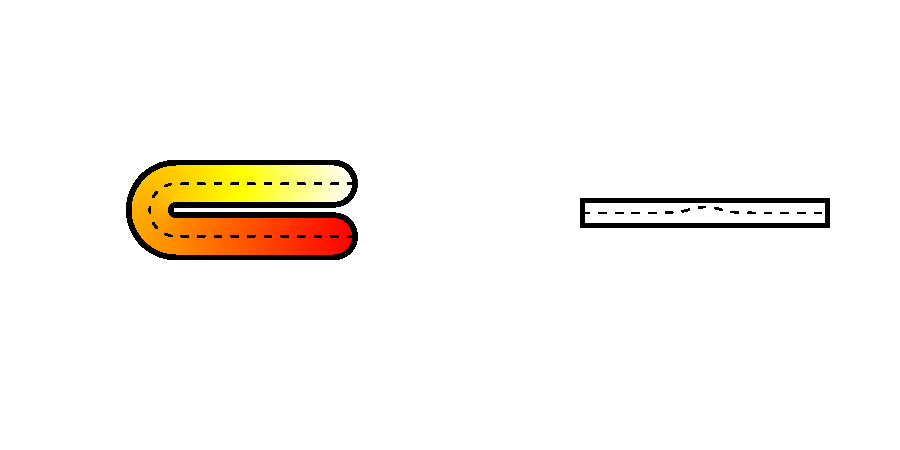
\includegraphics[trim=0.5in 1in 0in 1in]{figs/horseshoecentreline.pdf} \\
\caption{The dashed line here gives the centre line that we will map to investigate the smoothness under the \sch transform. The left figure gives the untransformed domain and the right the one that has undergone the transformation.}
\label{horseshoecentreline}
% generated by /phd-smoothing/ramseysim/nullspace.test.R 
\end{figure}


\begin{figure}
\centering
% trim order l b r t
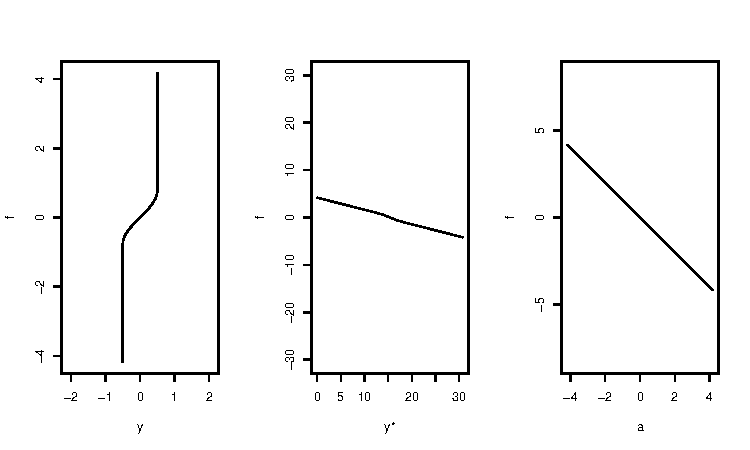
\includegraphics[trim=0in 0in 0in 0in]{figs/centrelinelineplots.pdf} \\
\caption{Plots of the horseshoe function against the $y$ axis for (left) the untransformed horseshoe, (middle) the shape under the \sch transform and, (right) the function evaluation against the major axis.}
\label{centrelinelineplot}
% generated by /phd-smoothing/ramseysim/nullspace.test.R 
\end{figure}

From these plots one can see that the \sch transform approximates the natural domain of the horseshoe quite well, with only two minor kinks in the line. Looking at where the kink occurs, it corresponds exactly with the kink in \fig{horseshoecentreline}. This makes sense, since we would expect a change in gradient if direction we are traveling has moved into two dimensions from one.

We now return to our original question of the nullspace of the penalty. The original Ramsay test function is given by a simple gradient in the direction of the major axis of the horseshoe. This function would not be penalized, as it is just a straight line (and hence its second derivative is zero.) We can see from \fig{centrelinelineplot} that in the natural domain of the horseshoe the line is straight and that this is almost the case in the transformed domain. Hence we can conclude that in this case the nullspace is almost the same as that in the natural domain.

In the next section we investigate the properties of the transform further via a simulation experiment.

\section{Simulations}

In the spirit of those simulations carried out in \cite{soap}, a large scale experiment was run. Data was simulated from two different test functions on the Ramsey horseshoe; first the one described above, and the second with a gradient across the short axis of the horseshoe. This second test function can be seen in \fig{altramsayhorseshoe}. Table (\ref{simtable}) shows the setup of these experiments, which were run on both test functions.

\begin{figure}
\centering
% trim order l b r t
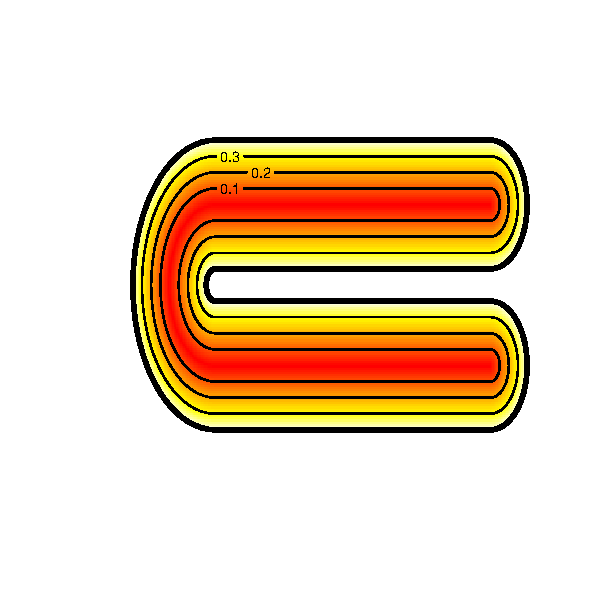
\includegraphics[trim=0.5in 1in 0in 0.5in]{figs/altramsayhorseshoe.pdf} \\
\caption{Heatmap of the alternate version of the Ramsay horseshoe.}
\label{altramsayhorseshoe}
\end{figure}

\begin{table}[ht]
\begin{tabular}{c c}\\
Sample size & Noise level$^{1}$ \\
\hline
\hline
1000 & 0.3 \\
500 & 0.3 \\
250 & 0.3 \\
100 & 0.3 \\
1000 & 0.5 \\
1000 & 1 \\
1000 & 2 \\
\end{tabular}
\caption{Setup for the simulations. $^{1}$Noise level is noise added to the test function from a standard Normal multiplied by the value in this column.}
\label{simtable}
\end{table}

Mean squared error between the true function and the fitted model was used to evaluate the model's performance. In the following tables we provide the mean squared error over a prediction grid of 1000 points averaged over 1000 generated data sets.

Table (2) shows the results from the simulations for the standard horseshoe. A cursory glance show that that results were better than those for the soap film smoother for larger sample sizes and standard errors were comparable. Indeed, once we get to 100 samples the method performance degrades significantly. However, this is not as bad as it initially seems to be. Only 6 of the 1000 MSEs were greater than the mean (the largest two being 54.6 and 437.99) so it seems that these two samples have contributed to significant departure from the mean. Given a different set of samples this problem may not manifest itself, however the soap film smoother still has a smaller MSE and standard error.

Once noise is introduced into the data we can see that the soap film and transformation method do as well as each other, MSEs are approximately the same and the standard errors are of the same order.

\begin{figure}
\centering
% trim order l b r t
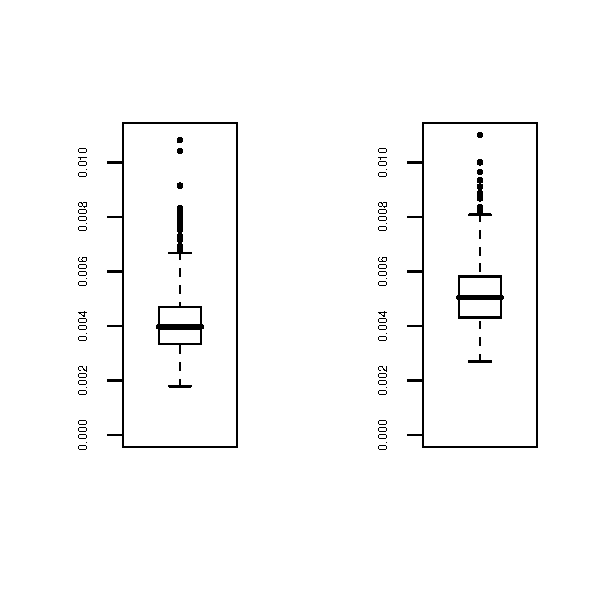
\includegraphics[trim=0.5in 1in 0in 0.5in]{figs/1000boxplots.pdf} \\
\caption{Boxplots of mean MSE from 1000 points on a prediction grid from 1000 simulations. Left plot is \sch transform with P-spline basis (with MSE 0.00412) and the right is the soap film smoother (MSE 0.00517.)}
\label{1000boxplots}
\end{figure}

\Fig{1000boxplots} compares boxplots of the MSEs for the first experiment. These plots show the \sch mapping doing better than the soap film smoother.

\begin{table}[ht]
\begin{tabular}{c c c c c}\\
Sample size & Noise level & P-spline MSE (\emph{se}) & Thin plate MSE (\emph{se}) & Soap MSE (\emph{se}) \\
\hline
\hline
1000 & 0.3 & 0.00412 (0.00112) & 0.00811 (0.00243) & 0.00517 (0.00114) \\ 
500 & 0.3 & 0.00505 (0.00144) & 0.00478 (0.000955) & 0.00628 (0.00146) \\ 
250 & 0.3 & 0.00875 (0.00392) & 0.00684 (0.00183) & 0.0107 (0.00305) \\ 
100 & 0.3 & 0.523 (14) & 0.0118 (0.00461) & 0.0219 (0.0117) \\ 
1000 & 0.5 & 0.0105 (0.00353) & 0.00811 (0.00243) & 0.0127 (0.0034) \\ 
1000 & 1 & 0.0242 (0.0108) & 0.0161 (0.0069) & 0.0275 (0.00958) \\ 
1000 & 2 & 0.066 (0.0481) & 0.0388 (0.0229) & 0.0686 (0.0333) \\ 
\end{tabular}
\label{table2}
\caption{Results table for the transformed Ramsay horseshoe.}
% generated by /phd-smoothing/sc-writeup/tablecode/ramsay.sim.results.table.R
\end{table}

For the alternative horseshoe we begin to see the soap film creep ahead of the transformation method (see table (3).) Although the MSEs are of approximately the same order (as are the standard errors), the soap film is gaining ground. To examine what is going on here we can look at the plots of the predicted values as heat maps. These can be seen in \fig{altramsaycomp} and show that the \sch mapping seems to capture the overall structure of the shape better than the soap film smoother, which seems to capture patches of the shape but not the overall structure. It also appears that the \sch method does not respect the ends of the horseshoe and continues the gradient running along the minor axis over this part as well.This feature seems to be the cause of the performance decrease.

\begin{table}[ht]
\begin{tabular}{c c c c c}\\
Sample size & Noise level & P-spline MSE (\emph{se}) & Thin plate MSE (\emph{se}) & Soap MSE (\emph{se}) \\
\hline
\hline
1000 & 0.3 & 0.00415 (0.00117) & 0.0158 (0.00247) & 0.00378 (0.00108) \\ 
500 & 0.3 & 0.00469 (0.00147) & 0.00793 (0.00186) & 0.00458 (0.00145) \\ 
250 & 0.3 & 0.00716 (0.00431) & 0.0142 (0.00249) & 0.00771 (0.00301) \\ 
100 & 0.3 & 0.039 (0.22) & 0.0201 (0.00589) & 0.0298 (0.42) \\ 
1000 & 0.5 & 0.00839 (0.00403) & 0.0158 (0.00247) & 0.00966 (0.00371) \\ 
1000 & 1 & 0.0194 (0.0122) & 0.0226 (0.0085) & 0.019 (0.00981) \\ 
1000 & 2 & 0.0605 (0.0468) & 0.0436 (0.0276) & 0.041 (0.0434) \\ 
\end{tabular}
\label{altramsayresultstable}
\caption{Results table for the transformed alternate Ramsay horseshoe.}
% generated by /phd-smoothing/sc-writeup/tablecode/alt.ramsay.sim.results.table.R
\end{table}

\begin{figure}
\centering
% trim order l b r t
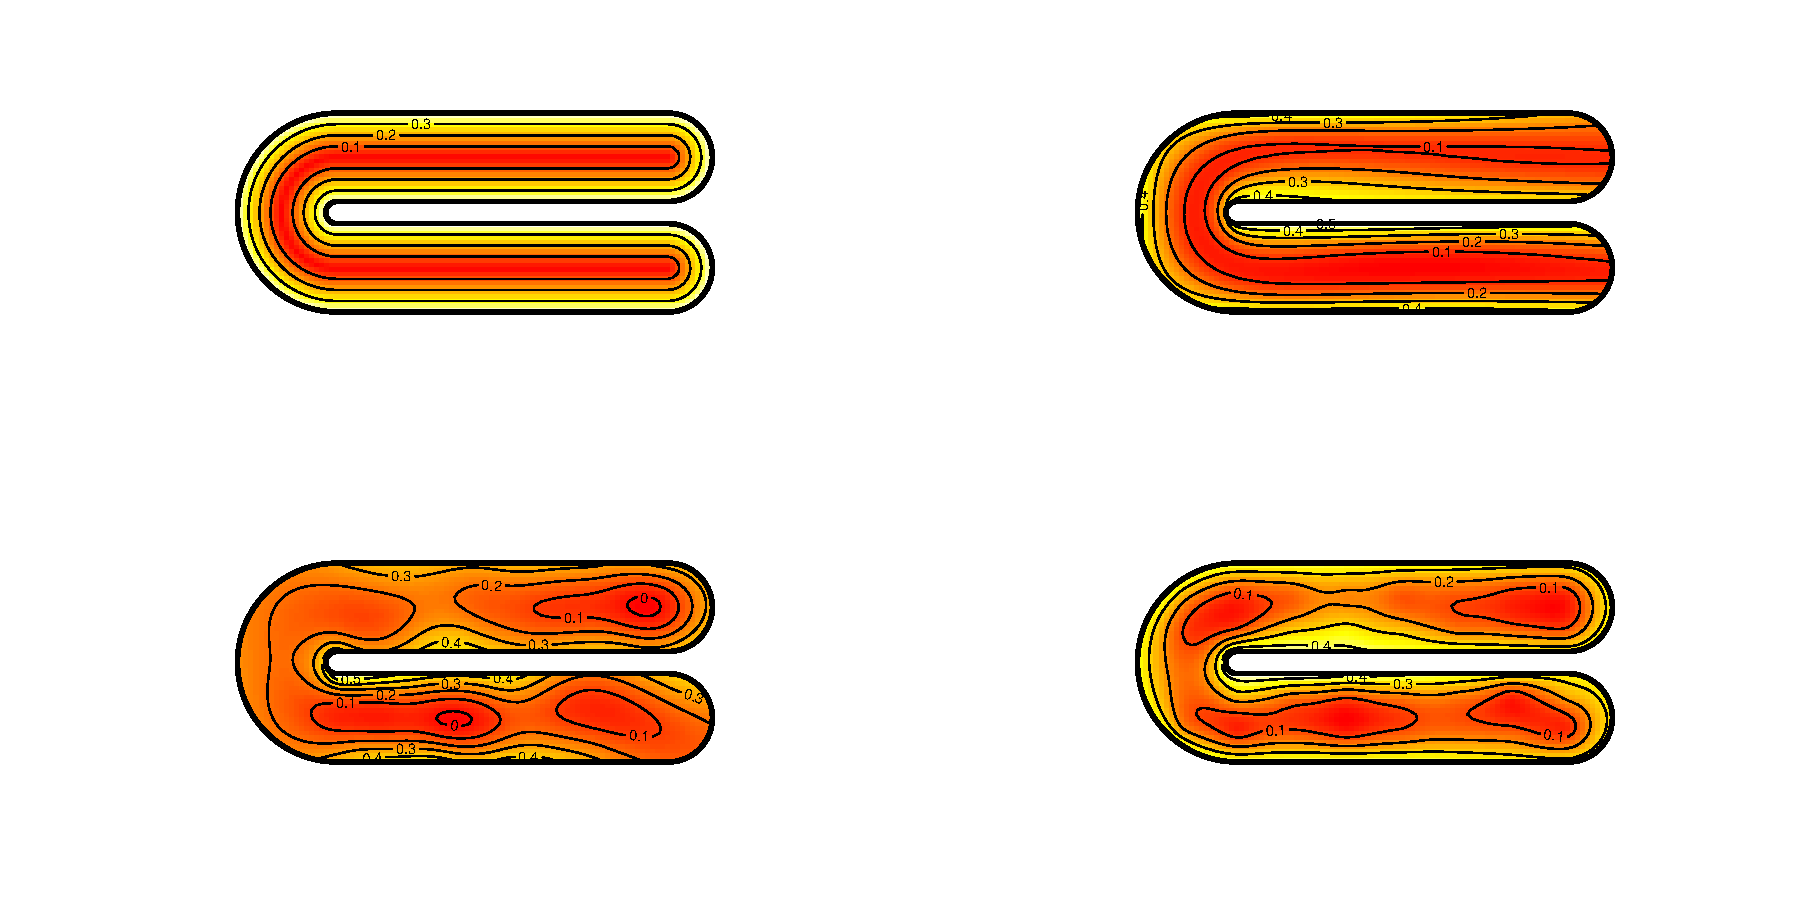
\includegraphics[width=5in, trim=0in 0in 0in 0in]{figs/altramsaycomp.pdf}\\
\caption{Clockwise from top left: the original figure, the function estimated by the \sch transform with P-splines, function estimated by the \sch transform with thin plate splines and finally the soap film estimate.}
\label{altramsaycomp}
% generated by /phd-smoothing/sc-writeup/figs/altramsaycompare.R 
\end{figure}

\Fig{altcentrelinelineplot} shows analogous plots to \fig{centrelinelineplot} and backs up this hypothesis. The second panel shows the mapping of the $y$ component of the centreline against the response and the third panel shows the same in the horseshoe's own domain. It appears that the two plots are indistinguishable.


\begin{figure}
\centering
% trim order l b r t
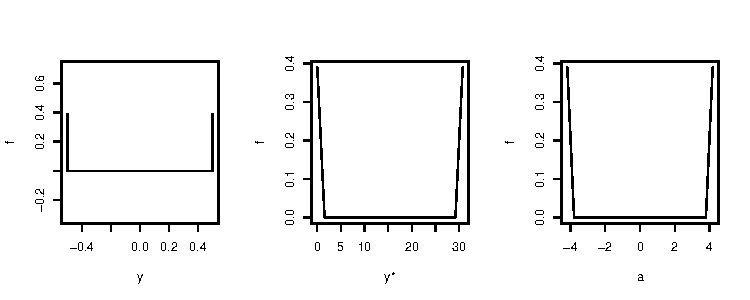
\includegraphics[trim=0in 0in 0in 0in]{figs/altcentrelinelineplots.pdf} \\
\caption{Plots of the alternate horseshoe function against the $y$ axis for (left) the untransformed horseshoe, (middle) the shape under the \sch transform and, (right) the function evaluation against the major axis.}
\label{altcentrelinelineplot}
% generated by /phd-smoothing/altramsaysim/nullspace.test.R 
\end{figure}


\section{Further work}

Using the \sch transform as an alternative method for smoothing via morphing the domain shows promise but is not without problems. The next steps are to first look at more difficult shapes in simulation and using real data to investigate the utility of the transform in practice. Secondly, in order to avoid the kind of problems discussed in the final section by using a better bounding box. Finally, it would be interesting to look at changing the penatly for the P-splines so that it relates to the distortion from the \sch transform. Such a penalty might take the form of being proportional to the ``area'' of a unit square in $W$ and $W^*$. This may then take into account the distortion of the space. This approach may allow for the distortions to be corrected for by undersmoothing areas that might be oversmoothed.




\bibliographystyle{plainnat}
\bibliography{sc-refs}



\end{document}
